%%%%%%%%%%%%%%%%%%%%%%%%%%%%%%%%%%%%%%%%%%%%%%%%%%%%%%%%%%%%%%%%%%
%%%%%%%% ICML 2015 EXAMPLE LATEX SUBMISSION FILE %%%%%%%%%%%%%%%%%
%%%%%%%%%%%%%%%%%%%%%%%%%%%%%%%%%%%%%%%%%%%%%%%%%%%%%%%%%%%%%%%%%%

% Use the following line _only_ if you're still using LaTeX 2.09.
%\documentstyle[icml2015,epsf,natbib]{article}
% If you rely on Latex2e packages, like most moden people use this:
\documentclass{article}

% use Times
\usepackage{times}
% For figures
\usepackage{graphicx} % more modern

%\usepackage{epsfig} % less modern
\usepackage{subfigure} 

% For citations
\usepackage{natbib}

% For algorithms
\usepackage{algorithm}
\usepackage{algorithmic}

% As of 2011, we use the hyperref package to produce hyperlinks in the
% resulting PDF.  If this breaks your system, please commend out the
% following usepackage line and replace \usepackage{icml2015} with
% \usepackage[nohyperref]{icml2015} above.
\usepackage{hyperref}

% Packages hyperref and algorithmic misbehave sometimes.  We can fix
% this with the following command.
\newcommand{\theHalgorithm}{\arabic{algorithm}}

% Employ the following version of the ``usepackage'' statement for
% submitting the draft version of the paper for review.  This will set
% the note in the first column to ``Under review.  Do not distribute.''
\usepackage{icml2015} 

% Employ this version of the ``usepackage'' statement after the paper has
% been accepted, when creating the final version.  This will set the
% note in the first column to ``Proceedings of the...''
%usepackage[accepted]{icml2015}


% The \icmltitle you define below is probably too long as a header.
% Therefore, a short form for the running title is supplied here:
\icmltitlerunning{Machine Learning Fall 2016 Programming Assignment 2}

\begin{document} 

\twocolumn[
\icmltitle{Machine Learning Fall 2016 Programming Assignment 2}

% It is OKAY to include author information, even for blind
% submissions: the style file will automatically remove it for you
% unless you've provided the [accepted] option to the icml2015
% package.
\icmlauthor{Alex Ring}{Alri7215@colorado.edu}
\icmladdress{CU Boulder, CO}

% You may provide any keywords that you 
% find helpful for describing your paper; these are used to populate 
% the "keywords" metadata in the PDF but will not be shown in the document
\icmlkeywords{boring formatting information, machine learning, ICML}

\vskip 0.3in
]
Alex Ring
\section{Functions Implemented}
The beta update function that I implemented was : $\beta[j] = \beta[j]' + \lambda(y_i - \pi_i)x_i$ where $\pi = \frac{exp(\beta^T x_i)}{1 + exp(\beta^t x_i)}$. The first step in my update is to index all of the non-zero values that we are passed from train example. I use this index to select values to update from the beta and x vectors respectively. Numpy allows us to index into their array objects with another array, this lets us update and select without a for loop, speeding up computation. I set the P variable (representing $\pi$ in the equation) and then set the step using the provided step function. Delta is set according to the beta update function above. I then go through and update the beta values for the entire vector. I decided to do this update before regularization because we don't always regularize and this saves computation in that case. The if statement following the update checks if $\mu$ is greater than 0. If $\mu$ is zero or less regularization does not make any sense, so we can skip the computation. The regularization itself happens in the for loop, I calculate shrinkage based on the $\lambda$ and $\mu$. I then use the last update variable to check the last time we updated to set my exponent correctly (m in the equation) and finally set the beta parameters with a second update using shrinkage and gap. In total the regularization update is:  $1 - (2\lambda\mu)^{m_j}$

\section{What is the role of the learning rate?}
The learning rate determines how far you are going to "step" in the gradient descent. Graphically it is how far down the curve you move from the previous iteration. Having a learning rate that is too large will result no convergence, a small learning rate takes long to converge. In short, the learning rate determines how fast we are converging towards optimal weights and how much the beta value is updated each pass. 

\section{How many passes over the data do you need to complete?} 
Three passes provided a 99\% accuracy on training data and a 94\% accuracy on test data. I would consider this acceptable. Results in table 1. 
\begin{table}[]
\centering
\caption{Passes over data}
\label{Passes}
\begin{tabular}{lllll}
Passes & TP          & HP         & TA       & HA       \\
1      & -112.590763 & -24.318733 & 0.964286 & 0.932331 \\
2      & -68.103173  & -19.901148 & 0.989662 & 0.939850 \\
3      & -52.946700  & -19.408414 & 0.996241 & 0.947368
\end{tabular}
\end{table}

\section{What words are good and bad predictors?}
Mathematically logistic regression pays more heed to words associated with larger beta weights. Essentially, $Class = \beta_1 x_1 +\beta_2 x_2 + . . .\beta_n x_n $ Larger beta values in the positive direction lead to a positive classification, and larger (negative) values in the negative direction lead to negative classification. Our data classifies baseball as positive and hockey as negative. We can easily find the best words for baseball by sorting the beta vector in ascending weight order and looking at the highest values. You can do the same to find the best hockey words by looking at the lowest values. 
\begin{table}[]
\caption{Good and bad predictors}
\label{}
\begin{tabular}{llllll}
         & 1        & 2       & 3    & 4        & 5      \\
Baseball & Pitching & Saves   & Bat  & Runs     & Hit    \\
Hockey   & Points   & Playoff & Pick & Playoffs & Hockey \\
Worst & Racist & Bloody & Blasted & Hooked & Intermissions
\end{tabular}
\end{table}
Mathematically the worst predictors of both classes are going to be the words that have beta weights of zero associated with them. A given $\beta_i x_i$ where $\beta$ = 0 will result in 0, causing no change in the calculation. Words that do this are the worst words for classification. You can find 0 values in the beta vector and the words associated with them. My results appear in table 2. 

\section{What happens to regularization if mu is 0?}
In Logistic regression the regularization part of the function is:  $1 - (2\lambda\mu)^{m_j}$ here we can see that if $\mu$ is equal to zero, the entire center part is going to be zero. So the function would simplify to one. (1 - 0) This would have no affect on the beta update because we would just be multiplying the beta parameter by one. Neither shrinking or enlarging it. 

\section{Extra Credit Vowpal Wabbit vs. Python Implementation}
I decided to compare the accuracy on test data with different numbers of passes over the data using both VW and this Python implementation. Overall Python preformed better and had a greater increase to accuracy with more passes. 

\begin{figure}
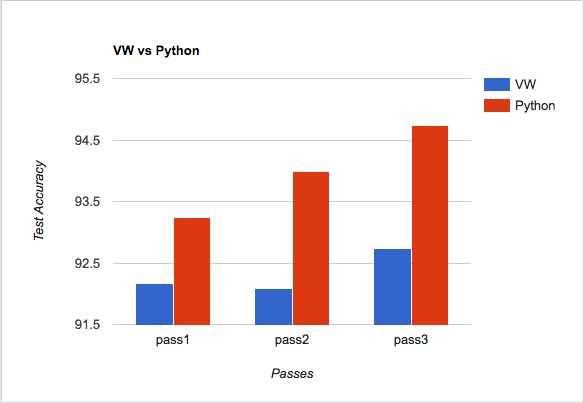
\includegraphics[scale=0.45]{graph}
\end{figure}

% In the unusual situation where you want a paper to appear in the
% references without citing it in the main text, use \nocite
\nocite{langley00}

\bibliography{example_paper}
\bibliographystyle{icml2015}

\end{document} 


% This document was modified from the file originally made available by
% Pat Langley and Andrea Danyluk for ICML-2K. This version was
% created by Lise Getoor and Tobias Scheffer, it was slightly modified  
% from the 2010 version by Thorsten Joachims & Johannes Fuernkranz, 
% slightly modified from the 2009 version by Kiri Wagstaff and 
% Sam Roweis's 2008 version, which is slightly modified from 
% Prasad Tadepalli's 2007 version which is a lightly 
% changed version of the previous year's version by Andrew Moore, 
% which was in turn edited from those of Kristian Kersting and 
% Codrina Lauth. Alex Smola contributed to the algorithmic style files.  
